
\section{かをり\index{かをり@かをり}という概念}
世の中には、様々な概念\index{がいねん@概念}が存在する。しかし、その概念\index{がいねん@概念}の範疇を越えようとしている概念が存在する。それこそまさに「かをり\index{かをり@かをり}」である。その概念\index{がいねん@概念}について詳しく述べる。

\subsection{爆誕}
 かをりという概念\index{がいねん@概念}が爆誕したのは1964年の12月25日である。奇しくもこの日は、あの伝説のアーティスト、オガワインティライミ\index{おがわいんてぃらいみ@オガワインティライミ}氏が生まれた日である6月24日から半年という、奇跡である。その上で、爆誕した日がクリスマスという、もはやイエスキリストという概念との比較すべき存在であることがわかる。\\
 ここで、LBFという存在を紹介する。LBF(University Bible Fellowship)とは大学生聖書読み宣協会のことで、なんか知らんけど謎の団体である。この団体の概念\index{がいねん@概念}はさておき、図\ref{ubf}を見ていただきたい。ここでは、コリント人への手紙が記されており、この「98-2講 私たちはキリストのかおり」には明確に「私達はキリストのかおり」と記してあるのである。念のため、この本文の一部を以下に示す。\\

\shadowbox{
\begin{tabular}{l}
98-2講 私達はキリストのかおり\\
 \\
投稿者: Jubfadmin 掲載日: 2004/12/23 (4352 回閲覧)\\
1998年コリント人への手紙第二 第2講\\
私達はキリストのかおり\\
 \\
御言葉:コリント人への手紙第二2:1?17\\
 \\
要 節:コリント人への手紙第二2:15\\
 \\
「私たちは、救われる人々の中でも、滅びる人々の中でも、神の前にかぐわしいキリストの\\
かおりなのです。」\\
今日の御言葉はクリスチャンの影響力に関する御言葉です。私達がどうすれば良い影響力を\\
及ぼすクリスチャンになれるでしょうか。今日の御言葉を通してその秘訣を学ぶことができる\\ように祈ります。\\
 \\
?。あふれるばかりの愛(1?11)\\
 第一に、涙の人、パウロ(1?4)。1節をご覧下さい。「そこで私は、あなたがたを悲し\\
ませることになるような訪問は二度とくり返すまいと決心したのです。」使徒パウロがコリント\\
教会を開拓して離れている間にコリント教会は分裂して党派に分かれ、パウロの権威を認めない\\
人達がいました。そのためにパウロは急いでコリント教会を訪問しましたが、事態は改善される\\
どころかますます悪化し、さすがのパウロも、悲しみを残して帰って来ました。それでパウロは彼\\
らを悲しませることになるような訪問は二度と繰り返すまいと決心しました。そのような状況では、\\
たとえ訪問しても、パウロもコリント人もお互いに悲しい思いをさせられるばかりだったからです。
\end{tabular}
}\\
 \\
 まず問題なのが、このコリント人への手紙が98-2まであるということである。長すぎるのである。しかも文字化けしているのである。カスカスカス\index{かす@カス}。そして、極めつけは「私達はキリストのかおり」という文章である。キリストという概念に対して「私達」という複数形の表現から、複数人の概念であることが推測される。そのくせに、キリストのかおりという概念に収束するのである。しかし、ここで注目したいのは「かおり」という表記である。我々が提示する概念は「かをり」であるため、このキリストのかおりはあくまで下位互換であり、手下であり、不完全体である。ここから完全なキリストのかをりになるべく、懸命な努力をしていくのである。\\

\begin{figure}[H]
  \centering
  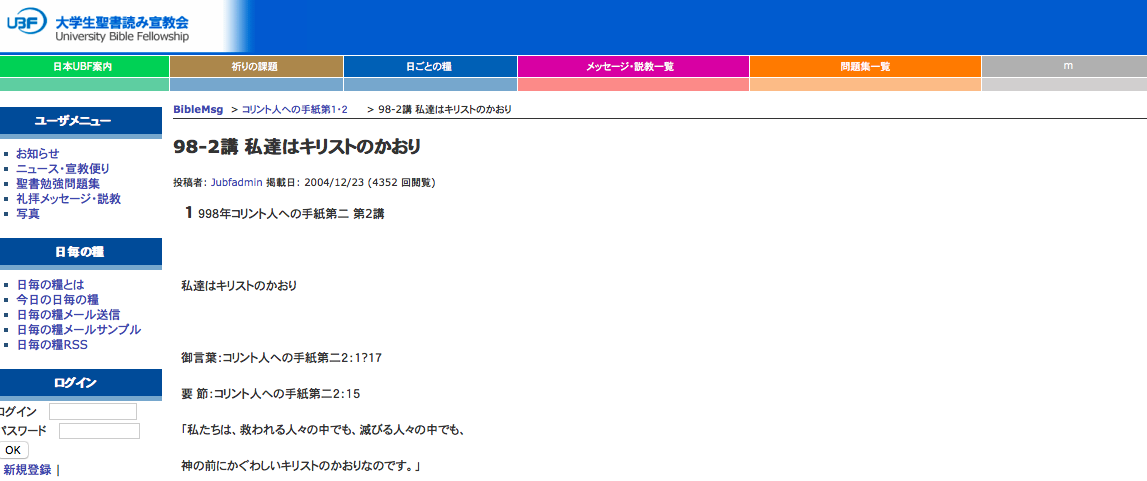
\includegraphics[clip,scale=0.4]{./section/Kawori/figures/ufb.png}
  \caption{投稿者: Jubfadmin 掲載日: 2004/12/23 (4352 回閲覧)}
\label{ufb}
\end{figure}

\subsection{世界デビュー}
ここからは、かをり\index{かをり@かをり}がかをりたる所以である。その存在が世界に明るみになった、デビューという概念が存在する。\\
事件が起こったのは2015年である。オガワインティライミ氏\index{おがわいんてぃらいみ@オガワインティライミ}が研究室にて爆誕した当初、その研究室ライフを謳歌すべく、自撮り棒の購入を試みた。どうせなら、公での購入であるため、研究室のパソコンを使用してAmazonを利用しようとした。図\ref{jidoribou}は当時、購入しようとした自撮り棒を同様のもののスクショを示す。

\begin{figure}[H]
  \centering
  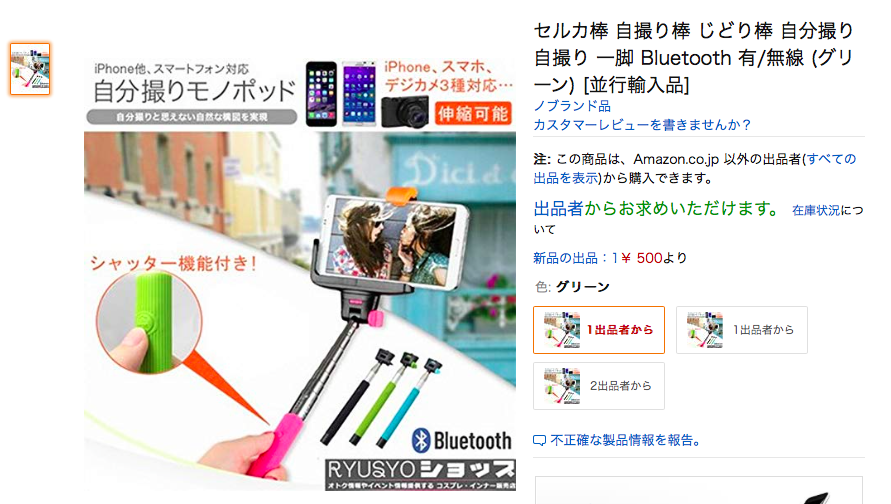
\includegraphics[clip,scale=0.4]{./section/Kawori/figures/jidoribou}
  \caption{値段は当時と変わらず500円という驚異的な安さである。また、自撮り棒の取っ手の部分がゴム製のカバーが付いており、写真などを撮るときにボタンを押す際にズレてなかなか撮影がうまくいかず、放送ジーコ監督就任のお知らせ\index{ほうそうじーこかんとくしゅうにんのおしらせ@放送ジーコ監督就任のお知らせ}である。}
\label{jidoribou}
\end{figure}

この破格的な値段から、即購入が決定したのだが、送り先を研究室にするために、発送先の設定をしようとしたところ、事件は起きたのである。購入手続きの流れで、宛先としてあの存在が表示されたのである。\\

\shadowbox{
\begin{tabular}{c}
オガワかをり
\end{tabular}
}

まさに、概念が概念を超えた瞬間である。この奇跡的な現象を観測したのは、世界を股にかける精鋭の研究部隊のメンバーであるタケダ氏\index{たけだ@タケダ}とグバ氏とオバ氏である。最新の記憶の呼び起こし研究の結果によると、その場にいたのがタケダ氏とグバ氏\index{ぐば@グバ}とオバ氏\index{おば@オバ}であるという。彼らによって、このオガワかをり現象は瞬く間に世界中に広まり、これが伝説的な世界デビューとなった。その後というものの、度々、風の噂でその伝説が誕生していき、その存在についてより活発な研究が進むこととなった。また、その存在を肉眼で一目見ようと、命知らずの重症患者\index{じゅうしょうかんじゃ@重症患者}達が死闘を繰り広げていくのである。




